\section{ROSMOD Tool Suite}
\label{sec:ROSMOD}

\subsection{Component Model}

Software development using ROSMOD is influenced by the principles of Component-based Software Engineering
\cite{CBSE}\cite{Heineman:01}. Large and complex systems are built by assembling reusable software pieces called \emph{components}. ROSMOD Components contain executable code that implement functions, manipulate state variables and interact with other components in the applications. This model is inspired by our previous efforts with the F6COM Component Model \cite{DREMS_CM}. The architecture of a ROSMOD component is shown in Figure \ref{fig:ROSMOD_Component}.

ROSMOD components can contain (1) publishers, (2) subscribers, (3) clients, (4) servers and (5) timers. Publisher ports publish (without blocking) messages of a message topic, and Subscriber ports subscribe to a message topic. Client ports require the services offered by server ports. Server ports provide services that can be used by the external world. Lastly, periodic and sporadic timers are used to trigger components. The semantics of these communication patterns are dictated by ROS.

To facilitate interactions with other components in an ordered manner, each component has a \emph{Component Message Queue}. This queue holds requests (i.e. messages) received from other interacting components or from the component's timers. %This queue supports a variety of scheduling schemes such as FIFO (first-in-first-out), PFIFO (priority-FIFO) and EDF (earliest-deadline-first) to enqueue received requests. 
These requests are processed by a single thread (per component) called the \emph{Component Executor Thread}. This thread is therefore responsible for executing all triggered callbacks e.g. subscriber callbacks, server callbacks and timer callbacks. 

\begin{figure}[h]
	\centering
	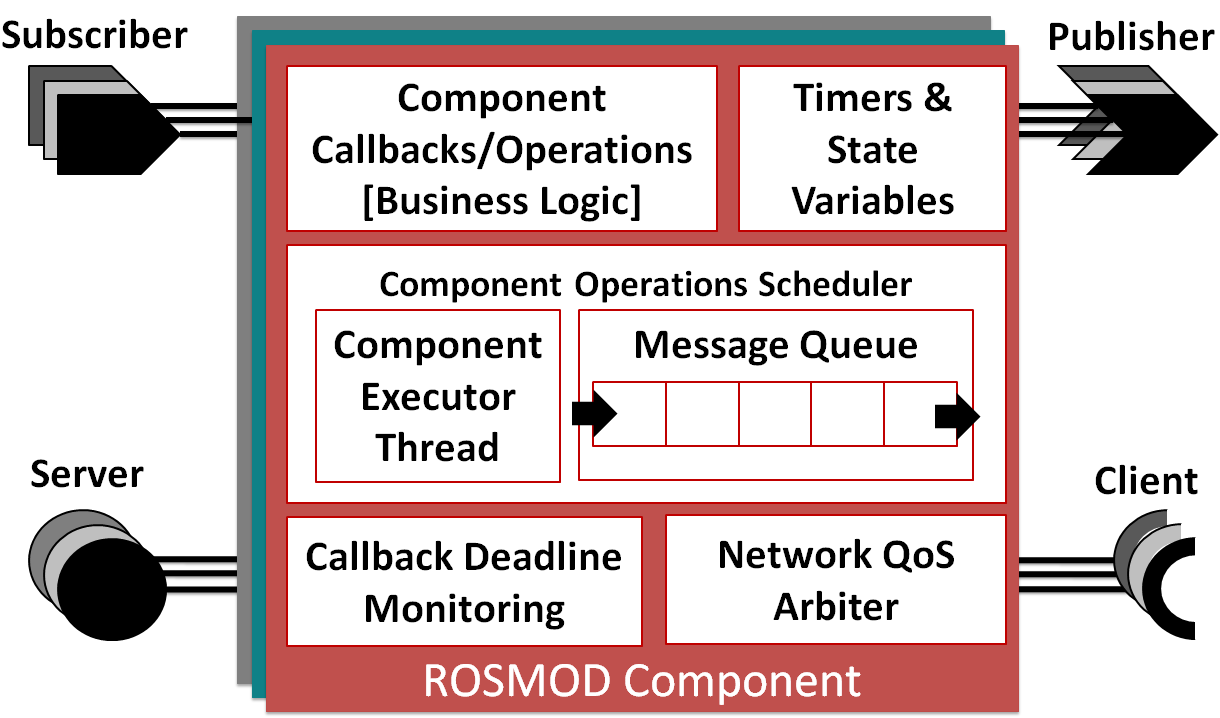
\includegraphics[width=0.45\textwidth]{figs/ROSMOD_Component.png}
	\caption{ROSMOD Component}
	\label{fig:ROSMOD_Component}
\end{figure}

\vspace{-0.1in}

Figure \ref{fig:Component_Message_Queue} shows a simple Client-Server component interaction. An Image Processor component is periodically triggered by a timer. At each timer expiry, this component, using its client port, makes a blocking remote procedure call to a Camera component. This service request is enqueued onto the Camera's message queue, and, when it reaches the front of the queue, the Camera component executor thread executes the corresponding server callback, returning the response to the Image Processor. This message queue-based interaction is also true for timers; when the timer in the Image Processor expires, a timer callback request is enqueued onto its message queue and eventually processed. 

\begin{figure}[h]
	\centering
	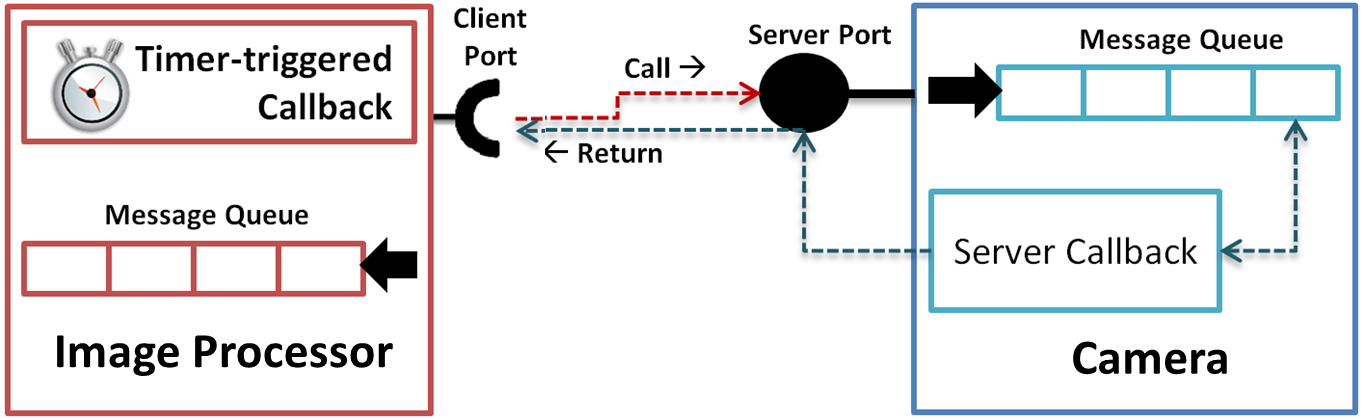
\includegraphics[width=0.48\textwidth]{figs/Component_Message_Queue.png}
	\caption{Component Interactions}
	\label{fig:Component_Message_Queue}
\end{figure}

It must be noted here that in each component, the message queue is processed by a single executor thread. Multiple components may run concurrently but each component's execution is single-threaded. Also, the component message queue supports several scheduling schemes including FIFO (first-in first-out), PFIFO (priority first-in first-out) and EDF (earliest deadline first). Requests in the message queue are processed using a non-preemptive scheduling scheme. This means that each callback/operation run by the executor thread is run to completion before the next one (waiting in the message queue) is processed. These rules are strictly applied to all ROSMOD components.

The single-threaded component execution is an important choice as it allows robust application development that is free of race conditions. Application integrators can avoid using synchronization primitives and locking mechanisms while developing code and this greatly simplifies design. These choices also more easily enable support for non-functional properties such as fault isolation and tolerance, operation timeliness and component lifecycle management. 

% ROS client library implementation called rosmod

\subsection{Modeling Language}

ROSMOD Projects are built using the ROSMOD Modeling Language. With this language, ROS users can create models of ROS workspaces, hardware topologies, deployment plans and more. The tool suite provides a Graphical User Interface to build these models but the state and configuration properties of the project are saved in a set of text files (models) that follow a strict set of grammatical rules, written using Antlr 4 \cite{ANTLR_BOOK}. Figure \ref{fig:ROSMOD_Project} shows the metamodel of the textual modeling language as a UML \cite{UML} class diagram.

\begin{figure*}[t]
	\centering	
	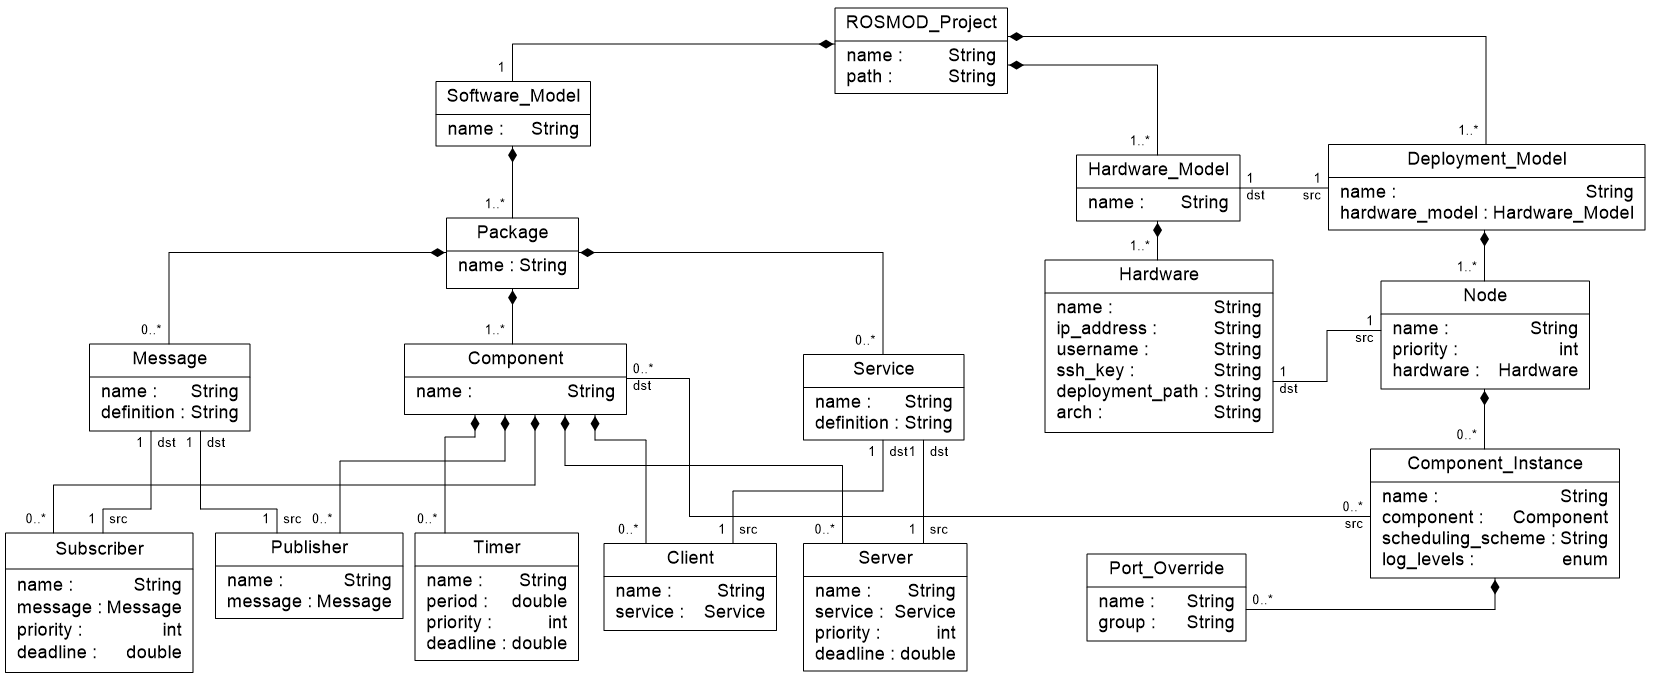
\includegraphics[width=1.0\linewidth]{figs/ROSMOD_Project.png}
	\caption{ROSMOD Project}
	\label{fig:ROSMOD_Project}	
\end{figure*}

\subsubsection{ROS Background}
ROS workspaces are high-level containers for source code which may contain one or more ROS packages.  ROS packages are containers which may include (1) one or more ROS message definitions for asynchronous publish/subscribe, (2) one or more ROS service definitions for synchronous RMI, and (3) one or more ROS Nodes, which are processes that can communicate with each other using predefined ROS messages or ROS services.  In this way a ROS package can be thought of as an application, and a ROS node is a process in that application.

\subsubsection{Software Model}
The ROSMOD Software model represents a ROS workspace. Each model consists of one or more ROS packages. Each ROS package contains definitions to (1) messages, (2) services and (3) components. The component assembly is derived from the interacting component ports. Ports that are associated with callbacks e.g. subscribers, contain both a \emph{priority} and a \emph{deadline} property to facilitate the scheduling schemes in the component model.

\subsubsection{Hardware Model}

Hardware models completely describe the hardware architecture of the system. Here, the user describes the different hardware hosts available for deployment, including their properties such as IP address, username and SSH keys.  These properties allow the user to directly map executables to hardware in a specified network and allow the deployment infrastructure to manage all remote operations and help ensure security between applications.  Deployment models refer to such predefined hardware models when mapping processes to hardware devices. Current work aims to improve on this hardware model by adding concepts for subnets, network interface controllers (NIC) and network links between hardware devices to more accurately represent the network topology.

\subsubsection{Deployment Model}

ROSMOD Deployment models contain the specifications for ROS nodes (executable processes). Each ROS node is ranked by a process priority and is mapped to a specific hardware device on which it will be executed. Each ROS node contains instances of software components that control its behavior. These component instances refer to specific components defined in the Software Model. At run-time, each node creates one executor thread per component instance before  beginning its interaction with the rest of the application. 

\paragraph{Group Assignment}
As shown in Figure \ref{fig:ROSMOD_Project}, each Component Instance can have \emph{port overrides}. These definitions override the ports previously defined in the Software Model. By assigning certain ports to a \emph{group}, a logical grouping of component ports is achieved. This ensures a strong coupling between ports. 

Suppose an \emph{ImageProcessor} client required a \emph{Camera} service, and this service was provided by two servers - \emph{LowResCamera} and \emph{HighResCamera}. Upon deployment, ROS typically couples the client with the server that advertises first. Although this is the default behavior, users can ensure a strong coupling between ports e.g. the ImageProcessor client connects only to the LowResCamera. This coupling overrides the default behavior, as seen in the Software Model.

\subsection{Graphical User Interface}

For large-scale applications, editing text files to describe ROSMOD Projects can be difficult and error prone, especially when referencing model objects defined in multiple files. To ease this development, we have built a Python-based graphical user interface, providing a rendering platform to quickly prototype models and understand the relationship between model elements e.g. component ports. 

This integrates well with our deployment infrastructure which opens up interfaces required to build ROS workspaces and deploy node executables. Users can build packages, copy deployment files,  \emph{start a deployment}, monitor running ROS nodes and open component instance-specific logs, all from the ROSMOD GUI.

\subsection{Generators} 

There are currently two classes of generators in ROSMOD. 

\subsubsection{Skeleton ROS Workspace}
\label{sec:generation}

The workspace generators produce a prototype skeleton ROS workspace. This includes (1) C++ classes for each ROSMOD component, (2) package-specific messages and services, (3) Logger and XML parser-specific files and (4) build system files, all organized following ROS package organization guidelines. Figure \ref{fig:Code_Generation} shows a sample generated code tree. This is the \emph{motor\_control} package used in our AGSE robot. There are three components - \emph{radial\_actuator\_controller}, \emph{vertical\_actuator\_controller} and a high-level \emph{servo\_controller}. The same figure shows the generated code specific to this package, organized following ROS package guidelines.

\begin{figure}[h]
	\centering
	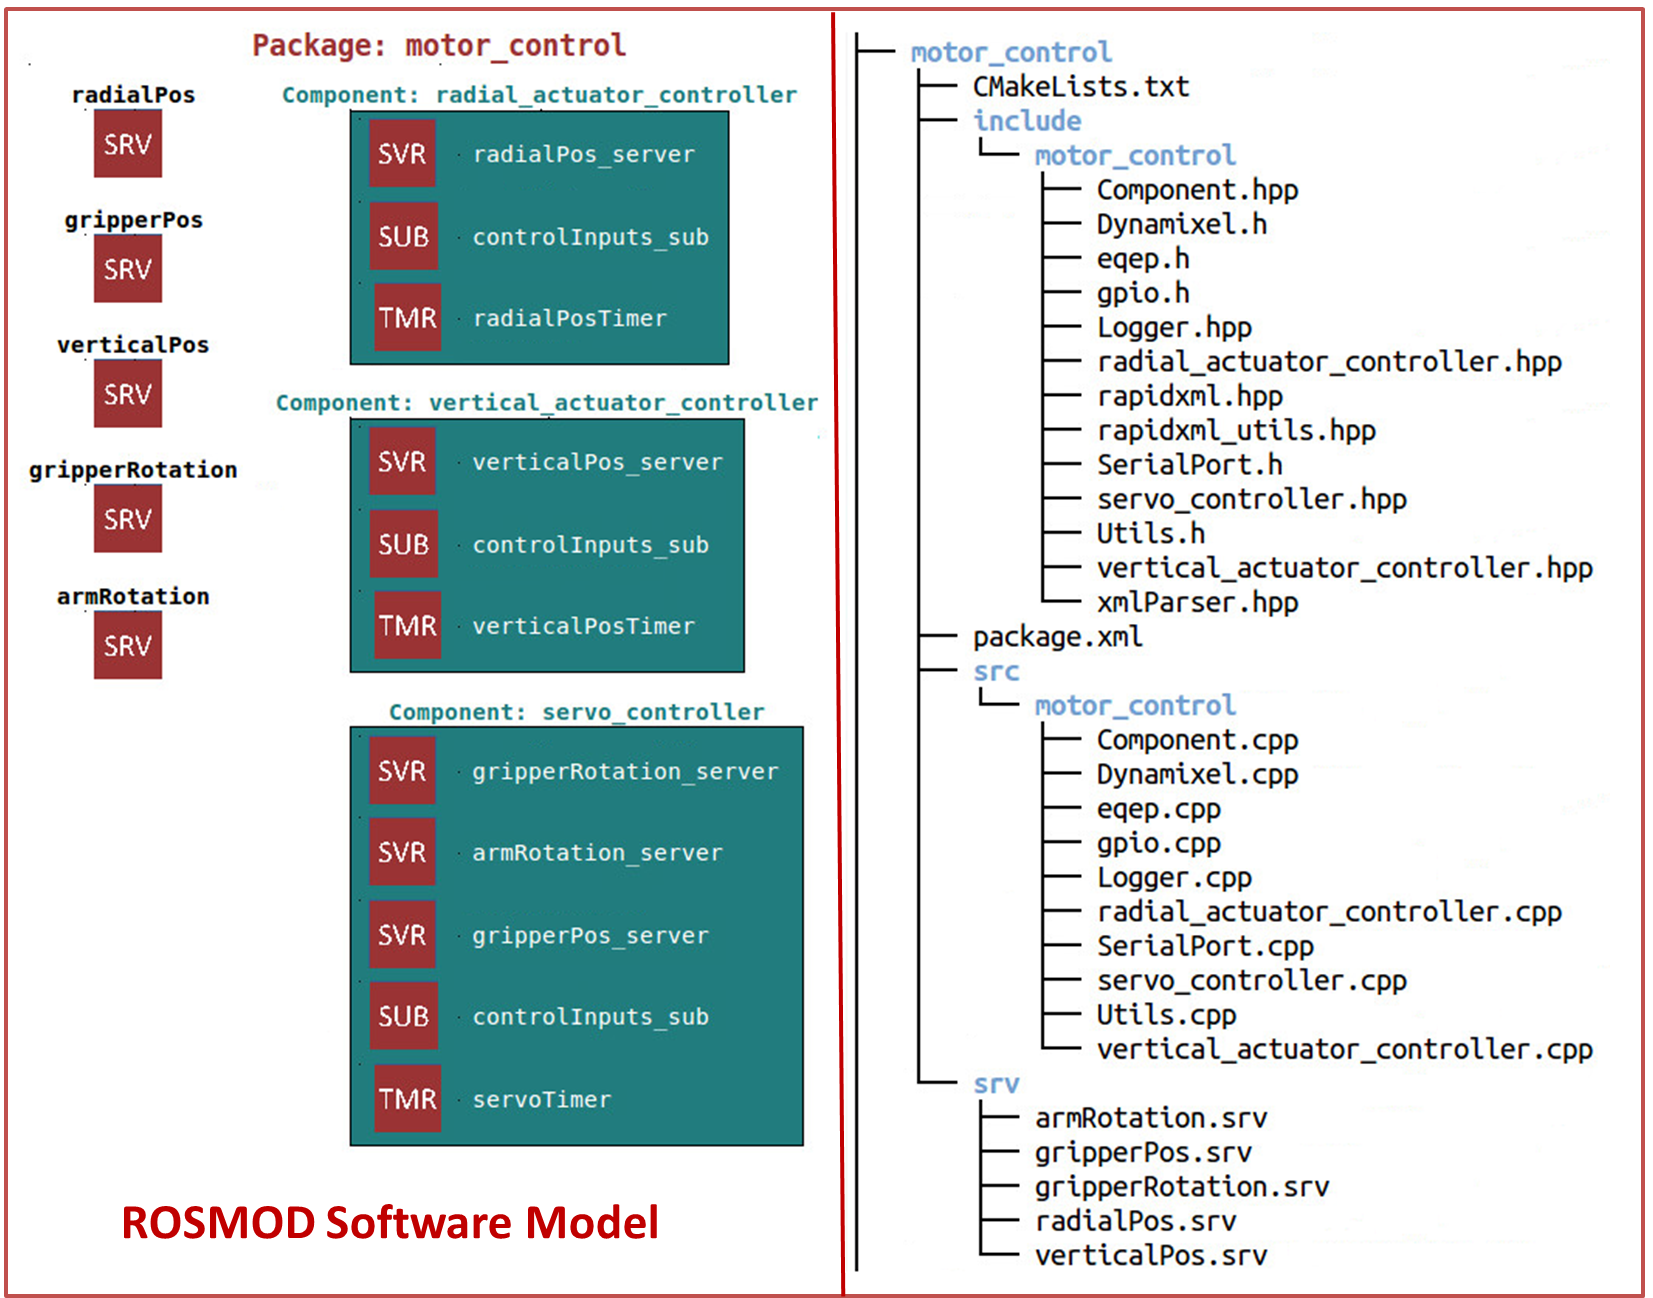
\includegraphics[width=0.50\textwidth]{figs/Code_Generation.png}
	\caption{Workspace Code Generation}
	\label{fig:Code_Generation}
\end{figure}

 In each package, the generated code includes code preservation markers around all callbacks and build system files so that users can quickly add new pieces of code which are guaranteed to be preserved after regeneration. This means that users can, for example, (1) generate a ROS workspace for a ROSMOD Software model, (2) add \emph{business logic} code in the generated skeleton callbacks, (3) go back to the models and add additional ports to specific ROSMOD components as required, and (4) regenerate the ROS workspace ensuring preservation of business logic code and selective code additions while accounting for the newly introduced ports. Therefore, users do not need to complete the ROSMOD models to begin C++ code development, enabling on-the-fly feature additions to ROS applications.

\subsubsection{Deployment-specific XML files}

The XML generators produce a batch of configuration files per deployment model. These files are fed to the node executable at run-time to easily change its behavior. Deployment-specific XML files contain properties of component instances in each ROS node, as seen in the deployment model in Figure \ref{fig:ROSMOD_Project}. It is typically desired to have knobs to easily tweak component properties e.g. message queue scheduling scheme, logging levels etc. at run-time without having to rebuild the ROS application. 

\subsection{Deployment Infrastructure}
\label{sec:Deployment_Infrastructure}

The workflow for software deployment is as shown Figure \ref{fig:workflow}. Every ROS workspace is generated with an additional \emph{node} package. This builds a generic node executable that can dynamically load libraries. Once the generators generate the ROS workspace and deployment XML files, users complete application development and build their ROS workspace. The build process generates dynamically loadable libraries, one for each component definition along with a single executable corresponding to the generic node package. The generated XML files contain metadata about about all ROS nodes modeled in the ROSMOD Deployment Model. This includes the component instances in each node and the appropriate component libraries to be loaded. Based on the XML file supplied to the node executable, the node will behave as one of the ROS nodes in the model. This allows for a reusable framework where a generic executable (1) loads an XML file, (2) identifies the component instances in the node, (3) finds the necessary component libraries to load and (4) spawns the executor threads bound to each component. 

\begin{figure}[h]
	\centering
	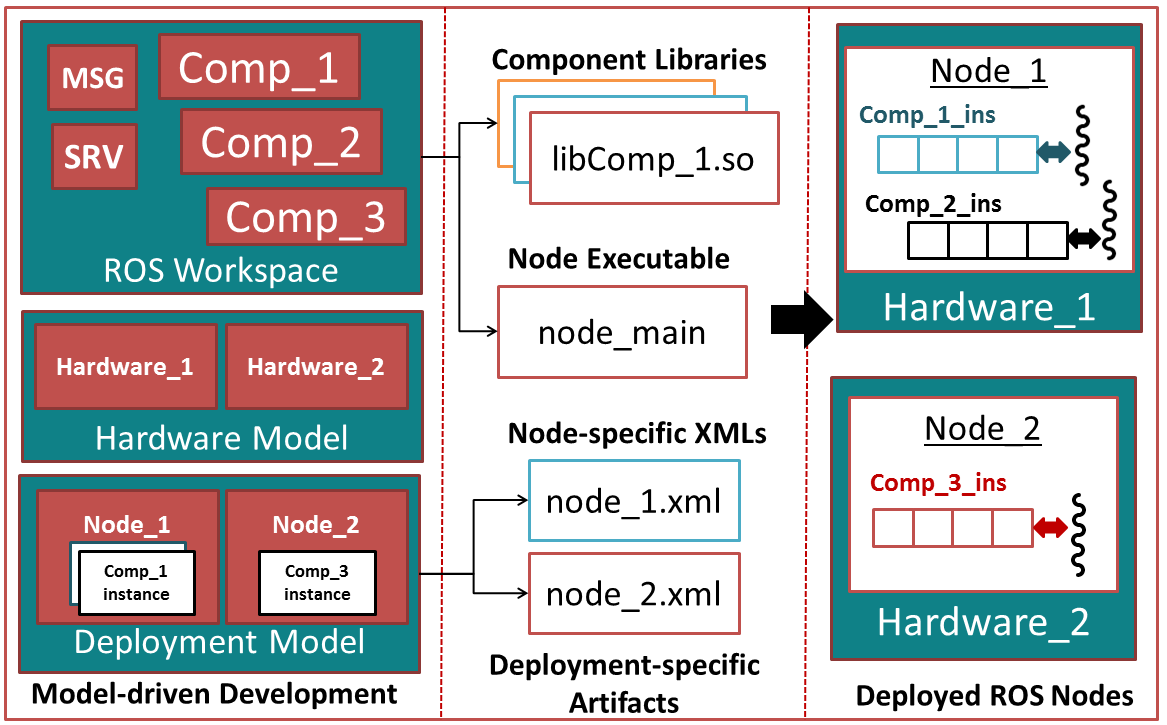
\includegraphics[width=0.50\textwidth]{figs/workflow.png}
	\caption{Software Deployment Workflow}
	\label{fig:workflow}
\end{figure}

In the above architecture, the deployment needs three primary ingredients: (1) the generic node executable, (2) dynamically loadable component libraries, and (3) an XML file for each ROS node in the deployment model. For each new node added to the deployment model, by merely regenerating the XML files, we can establish a new deployment. The ROS workspace is rebuilt only if new component definitions are added to the Software Model. This architecture not only accelerates the development process but also ensures a separation between the Software Model (i.e. the application structure) and deployment-specific concerns e.g. component instantiation inside ROS nodes.

%\subsection{run-time Logging}


%\subsection{Command Line Interface and Testing Framework}

%To automate testing requirements for applications while avoiding graphical strain on low-power embedded devices, ROSMOD also provides a command-line interface. Applications can be developed, built, deployed and managed using just the command line. This enables a testing framework that can be fully automated for large sets of ROSMOD projects as long as the deployment needs are met. This also enables testing a specific ROSMOD project repeatedly and in an automated manner for system-level properties such as timing violations, deadlocks, fault resilience and security requirements.